\documentclass[tikz,border=5]{standalone}
\usetikzlibrary{backgrounds,arrows.meta}
\begin{document}
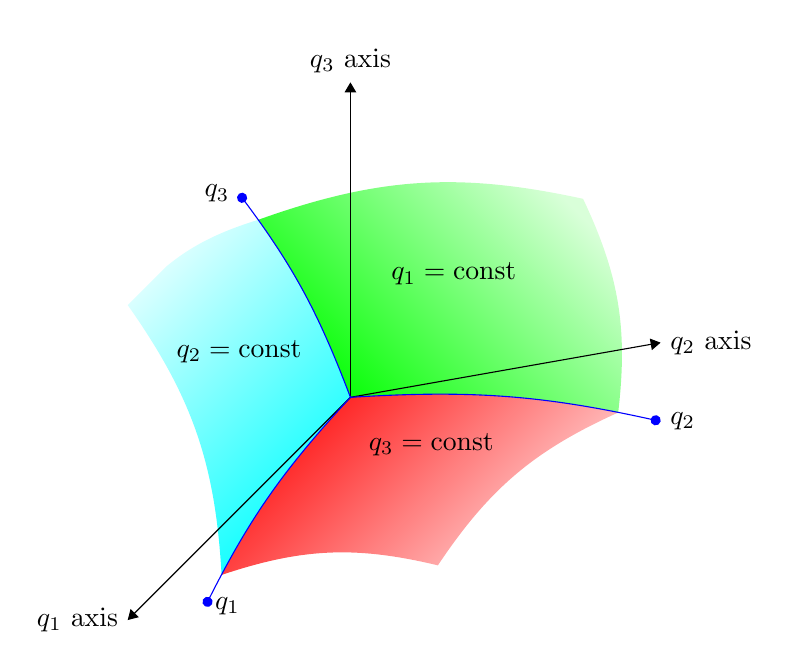
\begin{tikzpicture}[x=(10:4cm),y=(90:4cm),z=(225:4cm),>=Triangle]
\coordinate (O) at (0,0,0); 
\draw [->] (O) -- (1,0,0) node [at end, right] {$q_2$ axis};
\draw [->] (O) -- (0,1,0) node [at end, above] {$q_3$ axis};
\draw [->] (O) -- (0,0,1) node [at end, left]  {$q_1$ axis};

\draw [draw=blue, -Circle] (O) to [bend left=8] 
  coordinate [pos=7/8] (q2n) 
  (1,-1/4,0) coordinate (q2) node [right] {$q_2$};
\draw [draw=blue, -Circle] (O) to [bend right=8] 
  coordinate [pos=7/8] (q3n) 
  (0,1,1/2) coordinate (q3) node [left] {$q_3$};
\draw [draw=blue, -Circle] (O) to [bend right=8] 
  coordinate [pos=7/8] (q1n) 
  (1/4,0,1) coordinate (q1) node [right] {$q_1$};

\begin{pgfonlayer}{background}
\begin{scope}
\clip (O) to [bend left=8] (q2) -- (1,1,0) -- (q3n) to [bend right=8] (O);
\shade [left color=green, right color=green!15!white, shading angle=135]
  (O) to [bend left] (q3n) to [bend left=16] (3/4,1/2,0) to [bend left=16] (q2n) -- cycle;
\end{scope}

\begin{scope}
\clip (O) to [bend left=8] (q2) -- (1,0,1) -- (q1) to [bend left=8] (O);
\shade [left color=red, right color=red!15!white, shading angle=45]
  (O) to [bend right] (q1n) to [bend left=16] (1,0,1) to [bend left=16] 
  (q2n) to [bend right] (O);
\end{scope}

\begin{scope}
\clip (O) to [bend right=8] (q1) -- (0,1,1) -- (q3) to [bend left=8] (O);
\shade [left color=cyan, right color=cyan!15!white, shading angle=225] 
  (O) -- (q1n) to [bend right=16] (0,1,1) to [bend left=16] (q3n) 
to [bend left] (O);
\end{scope}
\end{pgfonlayer}

\node at (1/3,1/3,0) {$q_1=\mbox{const}$};
\node at (0,1/2,1/2) {$q_2=\mbox{const}$};
\node at (1/2,0,1/3) {$q_3=\mbox{const}$};
\end{tikzpicture}
\end{document}